% OSU Soundbendor Poster template.
% -- adapted from UMich template 
% -- https://www.overleaf.com/latex/templates/university-of-michigan-umich-poster-template/xpnqzzxwbjzc
% --
% -- Version 03-19-2026 by PJD

\documentclass[final]{beamer}

%=====================
% CHOOSE POSTER SIZE!
%=====================
%  Landscape 4'x3'
%---------------------
% Uncomment for Landscape
%\usepackage[orientation=landscape,width=4ft,height=3ft,scale=1.4]{beamerposter} 
%---------------------
%  Portrait A0
%---------------------
% Uncomment for Portrait
\usepackage[orientation=horizontal,size=a0,scale=1.4]{beamerposter}             
%---------------------

% ====================
% Packages
% ====================
\usepackage[T1]{fontenc}
\usepackage[utf8]{luainputenc}
\usepackage{lmodern}
\usepackage{style/osuposter}
\usepackage{style/colorosu}   % poster colors; palette from style/osucolors.sty (shared with slides)
\usepackage{graphicx}
\usepackage{booktabs}
\usepackage{tikz}
\usepackage{pgfplots}
\pgfplotsset{compat=1.14}
\usepackage{anyfontsize}

    
% ====================
% Lengths
% ====================
% If you have N columns, choose \sepwidth and \colwidth such that
% (N+1)*\sepwidth + N*\colwidth = \paperwidth
\newlength{\sepwidth}
\newlength{\colwidth}
\setlength{\sepwidth}{0.025\paperwidth}
\setlength{\colwidth}{0.3\paperwidth}
\newcommand{\separatorcolumn}{\begin{column}{\sepwidth}\end{column}}

% ====================
% Title
% ====================
% Set your title (subtitle optional)
\title{Some Fancy Title of the Poster:\\\textsl{followed by an optional subtitle}}
% Print the Author names
\author{Your Name}
% Institute name
\institute[OSU]{Oregon State University}


% ====================
% Footer (optional)
% ====================
% Footer content differs between Landscape and Portrait
% Set the Conference or Event Name below
% Comment out github or email to omit those fields, if desired
% Or freely type whatever you want within the footercontent{} block
\iflandscapeposter
    % Only present in Landscape size
    \footercontent{
        % Footer-left
        \href{https://github.com}{Github: https://github.com} \hfill 
        % Footer-middle
        \Large{\textbf{Conference Name}} \hfill
        % Footer-right
        \href{mailto:youremail@oregonstate.edu}{youremail@oregonstate.edu}
    }
\else
    % Only present in Portait size
    % Left is school logo; Right is lab logo
    \footercontent{
        % Footer-middle
        \Large{\textbf{Conference Name}} \hfill
    }
\fi
% (can be left out to remove footer)

% ====================
% Logo (optional)
% ====================
% use this to include logos on the left and/or right side of the header:

% Left: institution
 \logoleft{
\includegraphics[height=7cm]{style/logo/OSU-horizontal-white.png}}

% Right: funding agencies,lab, or other affilations 
\logoright{
\includegraphics[height=7cm]{style/logo/soundbendor-black-white.png}}

% ====================
% Body
% ====================
\begin{document}
\begin{frame}[t]
\begin{columns}[t]

\separatorcolumn
%====================
%---   COLUMN 1   ---
%====================
\begin{column}{\colwidth}

  %---------------------------------------------------------------------------
  \begin{block}{A block title}
  %---------------------------------------------------------------------------
    Some block contents, followed by a diagram, followed by a paragraph.

    \begin{figure}
      \centering
      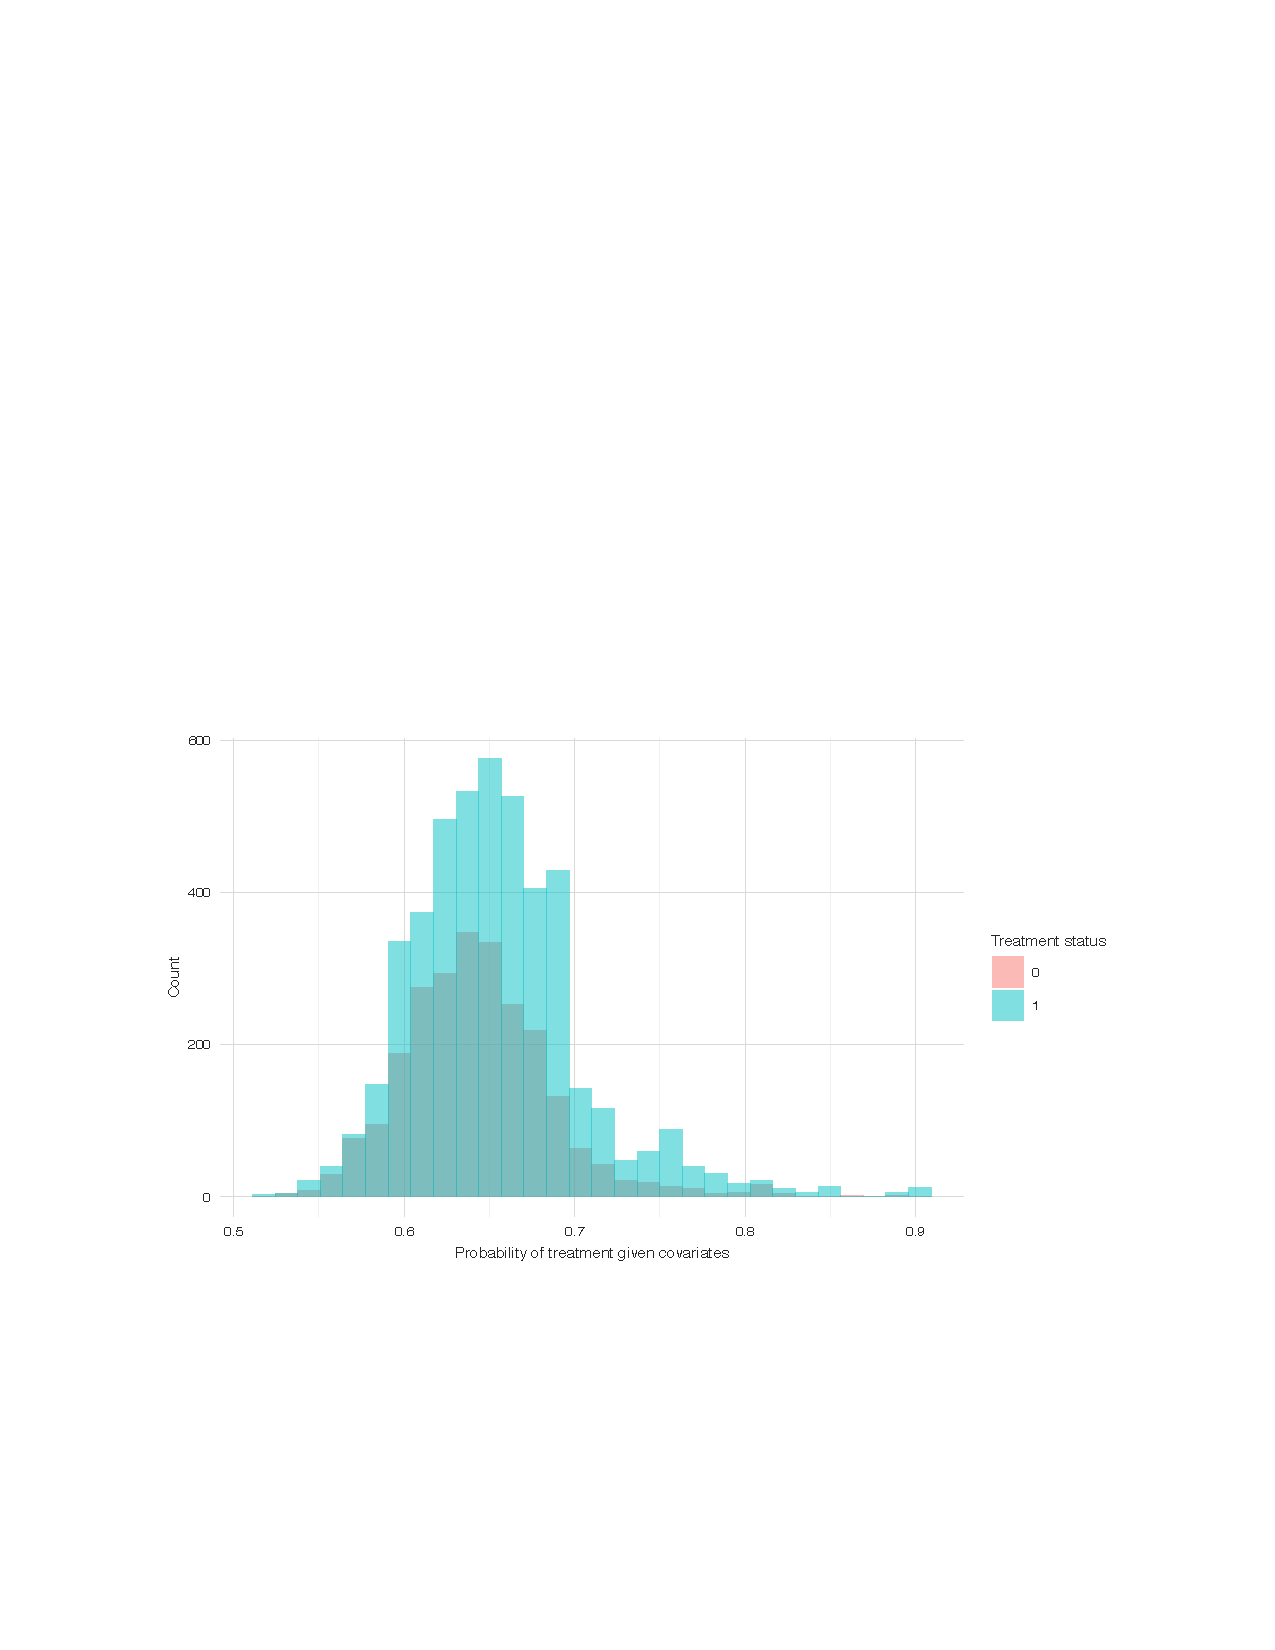
\includegraphics[width=0.6\textwidth]{figures/results_fig.pdf}
      \caption{A figure caption.}
    \end{figure}

    Lorem ipsum dolor sit amet, consectetur adipiscing elit. Morbi ultricies
    eget libero ac ullamcorper. Integer et euismod ante. 
    
  \end{block}
  %---------------------------------------------------------------------------
  
  %---------------------------------------------------------------------------
  \begin{block}{A block containing a list}
  %---------------------------------------------------------------------------
    Nam vulputate nunc felis, non condimentum lacus porta ultrices. 
    
    \begin{itemize}
      \item \textbf{Mauris tempor} risus nulla, sed ornare
      \item \textbf{Libero tincidunt} a duis congue vitae
      \item \textbf{Dui ac pretium} morbi justo neque, ullamcorper
    \end{itemize}

  \end{block}
  %---------------------------------------------------------------------------
  
  %---------------------------------------------------------------------------
  \begin{alertblock}{A highlighted block}
  %---------------------------------------------------------------------------
    This block catches your eye, so \textbf{important stuff} should go
    here.

    Curabitur eu libero vehicula, cursus est fringilla, luctus est. Morbi
    consectetur mauris quam, at finibus elit auctor ac. 

    \begin{itemize}
      \item \textbf{Fusce dapibus tellus} vel tellus semper finibus. In
        consequat, nibh sed mattis luctus, augue diam fermentum lectus.
      \item \textbf{In euismod erat metus} non ex. Vestibulum luctus augue in
        mi condimentum, at sollicitudin lorem viverra.
      \item \textbf{Suspendisse vulputate} mauris vel placerat consectetur.
        Mauris semper, purus ac hendrerit molestie, elit mi dignissim odio, in
        suscipit felis sapien vel ex.
    \end{itemize}

  \end{alertblock}
  %---------------------------------------------------------------------------
\end{column}

\separatorcolumn
%====================
%---   COLUMN 2   ---
%====================
\begin{column}{\colwidth}

  %---------------------------------------------------------------------------
  \begin{block}{A block with enumerated list}
  %---------------------------------------------------------------------------
    Vivamus congue volutpat elit non semper. Praesent molestie nec erat ac
    interdum. In quis suscipit erat. \textbf{Phasellus mauris felis, molestie
    ac pharetra quis}, tempus nec ante. Donec finibus ante vel purus mollis
    fermentum. Sed felis mi, pharetra eget nibh a, feugiat eleifend dolor. Nam
    mollis condimentum purus quis sodales. 
    
    %Nullam eu felis eu nulla eleifend bibendum nec eu lorem. 
    
    %Vivamus felis velit, volutpat ut facilisis ac,  commodo in metus.

    \begin{enumerate}
      \item \textbf{Morbi mauris purus}, egestas at vehicula et, convallis
        accumsan orci. Orci varius natoque penatibus et magnis dis parturient
        montes, nascetur ridiculus mus.
      \item \textbf{Cras vehicula blandit urna ut maximus}. Aliquam blandit nec
        massa ac sollicitudin. 
    \end{enumerate}

  \end{block}
  %---------------------------------------------------------------------------
  
  %---------------------------------------------------------------------------
  \begin{block}{Fusce aliquam magna velit}
  %---------------------------------------------------------------------------
    Et rutrum ex euismod vel. Pellentesque ultricies, velit in fermentum
    vestibulum, lectus nisi pretium nibh, sit amet aliquam lectus augue vel
    velit. Suspendisse rhoncus massa porttitor augue feugiat molestie. 

    \begin{figure}
      \centering
        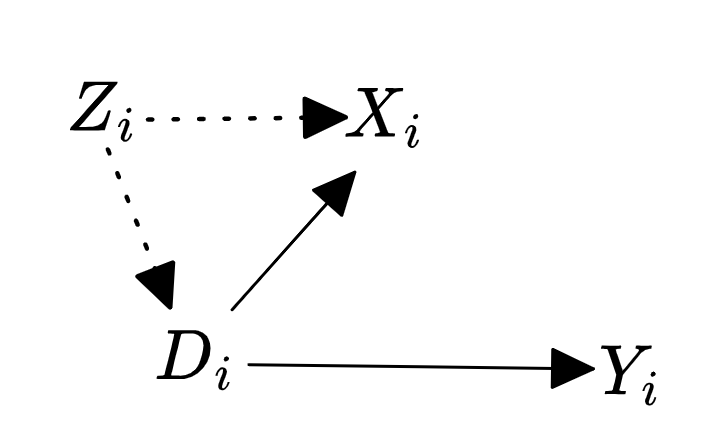
\includegraphics[width=0.3\textwidth]{figures/dag.png}

      \caption{Another figure caption.}
    \end{figure}

  \end{block}
  %---------------------------------------------------------------------------
  
  %---------------------------------------------------------------------------
  \begin{block}{Nam cursus consequat}
  %---------------------------------------------------------------------------
    Nulla eget sem quam. Ut aliquam volutpat nisi vestibulum convallis. Nunc a
    lectus et eros facilisis hendrerit eu non urna. Interdum et malesuada fames
    ac ante \textit{ipsum primis} in faucibus. 

    \begin{itemize}
      \item \textbf{Sed consequat} id ante vel efficitur. Praesent congue massa
        sed est scelerisque, elementum mollis augue iaculis.
        \begin{itemize}
          \item In sed est finibus, vulputate
            nunc gravida, pulvinar lorem. In maximus nunc dolor, sed auctor eros
            porttitor quis.
            \begin{itemize}
                \item Fusce ornare dignissim nisi. Nam sit amet risus vel lacus
            tempor tincidunt eu a arcu.
                \item Donec rhoncus vestibulum erat, quis aliquam leo
            gravida egestas.
            \end{itemize}
        \end{itemize}
      \item \textbf{Sed luctus, elit sit amet} dictum maximus, diam dolor
        faucibus purus, sed lobortis justo erat id turpis.
    \end{itemize}

  \end{block}
  %---------------------------------------------------------------------------
\end{column}

\separatorcolumn
%====================
%---   COLUMN 3   ---
%====================
\begin{column}{\colwidth}

  %---------------------------------------------------------------------------
  \begin{exampleblock}{A highlighted block containing some math}
  %---------------------------------------------------------------------------
    A different kind of highlighted block.

    $$
    \int_{-\infty}^{\infty} e^{-x^2}\,dx = \sqrt{\pi}
    $$

    Interdum et malesuada fames $\{1, 4, 9, \ldots\}$ ac ante ipsum primis in
    faucibus. Cras eleifend dolor eu nulla suscipit suscipit. 

    \heading{A heading inside a block}

    Praesent consectetur mi $x^2 + y^2$ metus, nec vestibulum justo viverra
    nec. Proin eget nulla pretium, egestas magna aliquam, mollis neque. Vivamus
    dictum $\mathbf{u}^\intercal\mathbf{v}$ sagittis odio, vel porta erat
    congue sed. Maecenas ut dolor quis arcu auctor porttitor.

    \heading{Another heading inside a block}

    Sed augue erat, scelerisque a purus ultricies, placerat porttitor neque.
    Donec $P(y \mid x)$ fermentum consectetur $\nabla_x P(y \mid x)$ sapien.

  \end{exampleblock}
  %---------------------------------------------------------------------------
  
  %---------------------------------------------------------------------------
  \begin{block}{Nullam vel erat at velit convallis laoreet}
  %---------------------------------------------------------------------------
    Class aptent taciti sociosqu ad litora torquent per conubia nostra, per
    inceptos himenaeos. Phasellus libero enim, gravida sed erat sit amet,
    scelerisque congue diam. Fusce dapibus dui ut augue pulvinar iaculis.

    \begin{table}
      \centering
      \begin{tabular}{l c c c}
        \toprule
        \textbf{First} & \textbf{Second} & \textbf{Third} & \textbf{Fourth} \\
        \midrule
        Foo & 13.37 & 384,394 & $\alpha$ \\
        Bar & 2.17 & 1,392 & $\beta$ \\
        Baz & 3.14 & 83,742 & $\delta$ \\
        Qux & 7.59 & 974 & $\gamma$ \\
        \bottomrule
      \end{tabular}
      \caption{A table caption.}
    \end{table}

  \end{block}
  %---------------------------------------------------------------------------
  
  %---------------------------------------------------------------------------
  \begin{block}{References}
  %---------------------------------------------------------------------------
    \nocite{*}
        \vspace{-3mm}
        \footnotesize{\bibliographystyle{unsrt}\bibliography{poster}}

  \end{block}
  %---------------------------------------------------------------------------
  
\end{column}

\separatorcolumn
\end{columns}
\end{frame}

\end{document}